\documentclass[12pt]{article}

% Packages
\usepackage{amssymb}
\usepackage{amsmath} % align
\usepackage{xcolor}
\usepackage{graphicx}
\usepackage{subfig}
\usepackage{multirow}
\usepackage{centernot}
\usepackage{setspace}

\usepackage{tikz}


\DeclareMathOperator*{\argmin}{arg\,min}


\begin{document}

\newcommand{\comm}[1]{}

\newcommand{\mb}{\mathbf}

\section{Posterior probability - Log likelihood {\small(PP-LL)}} \label{sec:loglik} %%%%%%%%%%%%%%%%%%%%%%%%%%%%%%%%%%%%

\subsection{Background} 

\subsubsection*{Reading list} %%%%%%%%%%%%%%%%%%%%%%%%%%%%%%%%%%%%%%%%%%%%%%%%%%%%%%%
Non-negative matrix factorization \cite{Lee1999Learning}. 
Divergences for exponential families \cite{Banerjee2005Clustering}.
Linear regression  \cite[ch 12.3]{Casella2002Statistical}.  
Association mining \cite{Agrawal1993Mining}.

\subsubsection*{Assumptions on $\mathbf{X}$} %%%%%%%%%%%%%%%%%%%%%%%%%%%%%%%%%%%%%

$\mathbf{X}_{n \times d}$ is the observed binary matrix with entries
\begin{align}
  x_{ij} &= 
  \begin{cases}
   1 &  \text{ if gene $j$ is expressed in cell $i$} \\
   0 & \text{ otherwise.}
  \end{cases}
\end{align}
Assume that the entries $x_{ij}$ are observations from $X_{ij}$  independent (but not identical) Bernoulli$(\pi_{ij})$ variables, where $\pi_{ij}$ is the probability of the $j$th gene in the $i$th cell being expressed. 
Assume that there exists an underlying binary structure matrix $\mathbf{S}_{n \times d}$, and define the relationship between  $\mathbf{X}$ and  $\mathbf{S}$ as follows

\begin{align} \label{eg: Xassumptions}
   \pi_{ij} &= (1 -  p_{ij}) + (2  p_{ij} - 1) s_{ij} \\
   p_{ij} & =  Pr(X_{ij} = s_{ij}) \nonumber
\end{align}
where $Pr$ is the probability function, and $s_{ij}$ are the entries of $\mathbf{S}$.

\subsubsection*{Assumptions on $\pi_{ij}$} %%%%%%%%%%%%%%%%%%%%%%%%%%%%%%%%%%%%%%%%%%%%%%%%%%%%%%%
Assume that $\pi_{ij}$ is a function of $s_{ij}$ as follows
\begin{align} \label{eq:Link}
  & \pi_{ij}(s_{ij}) = \frac{e^{\alpha_{ij} + \beta_{ij} s_{ij}}}{1 + e^{\alpha_{ij} + \beta_{ij} s_{ij}}}, \\
 \text{ which is equivalent to } \nonumber \\
  & \log \frac{\pi_{ij}(s)}{1-\pi_{ij}(s)}  = \alpha_{ij} + \beta_{ij} s_{ij},  \nonumber
\end{align}
and note that
\begin{align} \label{eq:p_alpha_pi}
  & p_{ij} =  \frac{1}{1 + e^{\alpha_{ij}}} =  \frac{e^{\alpha_{ij} + \beta_{ij}}}{1 + e^{\alpha_{ij} + \beta_{ij}}} \\
  & \pi_{ij}(1)  = 1 - \pi_{ij}(0). \nonumber
\end{align}

\subsubsection*{Problem definition} %%%%%%%%%%%%%%%%%%%%%%%%%%%%%%%%%%%%%%%%%%%%%
We want to find the underlying structure matrix $\mathbf{S}$ because we believe that this will give us information about how the cells and the genes in $\mathbf{X}$ cluster. 

\begin{center}
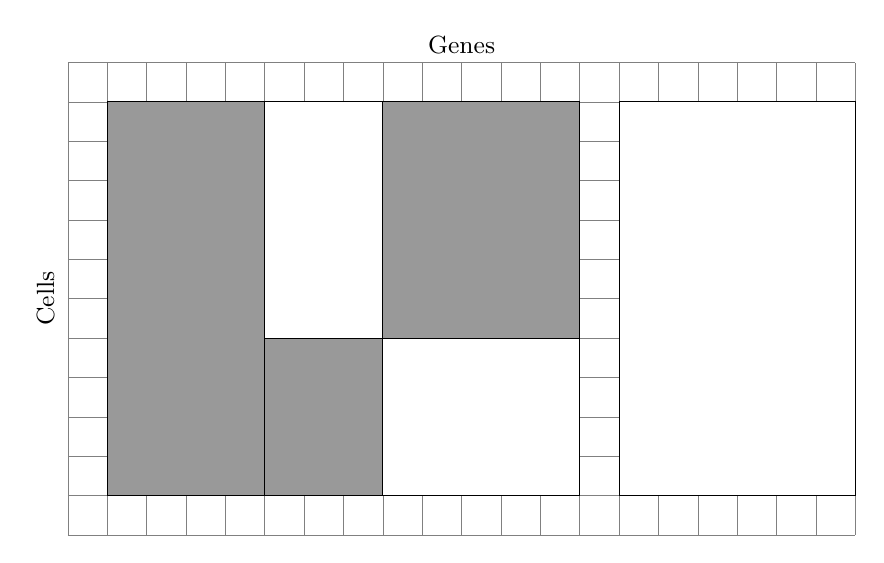
\begin{tikzpicture}
  \draw[step=0.5cm,gray,very thin] (0,0) grid (10,6);
   \filldraw[fill=black!40!white, draw=black] (0.5,5.5) rectangle (2.5,0.5);
   \filldraw[fill=white!40!white, draw=black] (2.5,5.5) rectangle (4,2.5);
  \filldraw[fill=black!40!white, draw=black] (2.5,2.5) rectangle (4,0.5);
  \filldraw[fill=black!40!white, draw=black] (4,5.5) rectangle (6.5,2.5);
  \filldraw[fill=white!40!white, draw=black] (4,2.5) rectangle (6.5,0.5);
  \filldraw[fill=white!40!white, draw=black] (7,5.5) rectangle (10,0.5);

  \node[below=0.8cm] at (5,7.25) {\small Genes};
  \node[rotate=90, above=0.8cm] at (0.75,3) {\small Cells};
\end{tikzpicture}
\vspace{2mm} \\
%\comm{
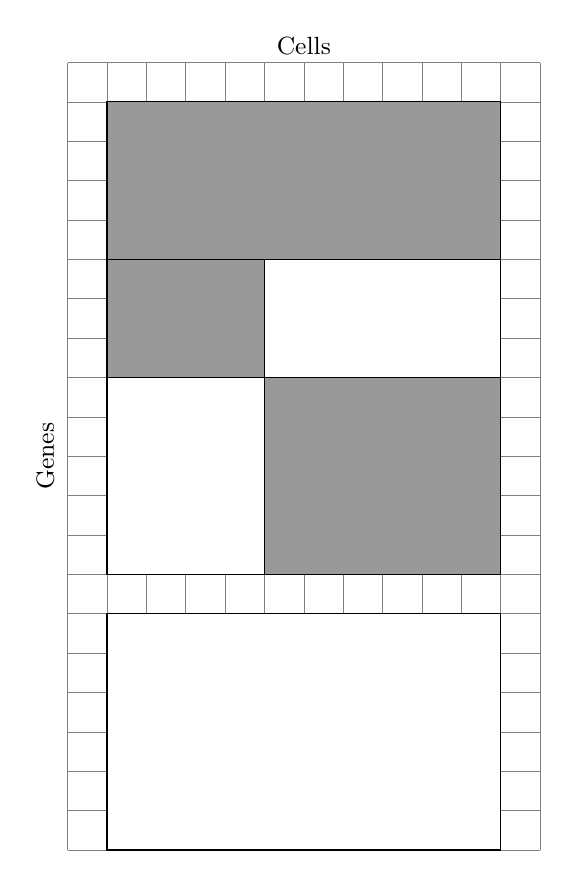
\begin{tikzpicture}
  \draw[step=0.5cm,gray,very thin] (0,0) grid (6,10);
   \filldraw[fill=black!40!white, draw=black] (0.5,9.5) rectangle (5.5,7.5);
   \filldraw[fill=black!40!white, draw=black] (0.5,7.5) rectangle (2.5,6);
  \filldraw[fill=white!40!white, draw=black] (2.5,7.5) rectangle (5.5,6);
  \filldraw[fill=white!40!white, draw=black] (0.5,6) rectangle (2.5,3.5);
  \filldraw[fill=black!40!white, draw=black] (2.5,6) rectangle (5.5,3.5);
  \filldraw[fill=white!40!white, draw=black] (0.5,3) rectangle (5.5,0);

  \node[below=0.8cm] at (3,11.25) {\small Cells};
  \node[rotate=90, above=0.8cm] at (0.75,5) {\small Genes};
\end{tikzpicture}
%}

\end{center}
Let $\mathbf{A}$ be a binary approximation of $\mathbf{S}$.
Finding  $\mathbf{S}$ is done by alternating between the two following steps \\
{\bf Step 1:} Estimate $\alpha_{ij}$ and $\beta_{ij}$, given $\mathbf{A}$. \\
{\bf Step 2:} Find a low rank approximation matrix $\mathbf{A}$ to $\mathbf{S}$, given the estimates of $\alpha_{ij}$ and $\beta_{ij}$. \\
We do this by replacing $\mathbf{S}$ by $\mathbf{A}$ to estimate $\alpha_{ij}$ and $\beta_{ij}$, and then use the estimates to find a new approximation $\mathbf{A}$, alternating between step 1 and step 2 until convergence or exhaustion. 
To avoid tendonitis, we will use $\alpha_{ij}$ and $\beta_{ij}$ for the estimated parameters, and $\mathbf{A}$ will denote any version of the approximation matrix, unless it is a necessity to distinguish between them. 

\subsection{Estimation of $\alpha_{ij}$ and $\beta_{ij}$, approximation of $\mathbf{S}$} %%%%%%%%%%%%%%%%%%%%%%%%%%%%%%%%%%%%%%%%

\subsubsection*{No cell effect, no gene effect} %%%%%%%%%%%%%%%%%%%%%%%%%%%%%%%%%%%%%%%%%%%%%%%%%%%

{\bf Step 1:} If we assume that $Pr(X_{ij} = s_{ij})$ is a constant $p$, i.e.\ no cell or gene effect, then we can then estimate $\alpha$ and $\beta$ using
\begin{align} \label{eq:AlphaBeta}
  \frac{\partial}{\partial \alpha} \log L(\alpha, \beta|\mathbf{X}) &= \sum_{i j} \big (x_{i j} - \pi(a_{ij}) \big) = 0 \\
  \frac{\partial}{\partial \beta} \log L(\alpha, \beta|\mathbf{X}) &= \sum_{i j} \big (x_{i j} - \pi(a_{ij}) \big )a_{ij} = 0. \nonumber
\end{align}

{\bf Step 2:} We will use the maximum likelihood to find $\mathbf{A}$. 
Recall that $P(X = x|\pi) = \pi^x (1 - \pi)^{(1-x)}$.
We want to maximize the likelihood function:
\begin{align}
  L \big (\pi(a_{ij})|\mathbf{X} \big ) =\prod_{i j}  \big ( \pi(a_{ij}) \big )^{x_{ij}} \big ( 1 - \pi(a_{ij}) \big) ^{1 - x_{ij}},
\end{align}
which is equivalent to maximizing the log likelihood
\begin{align}
  \log L \big (\pi(a_{ij})|\mathbf{X} \big ) =\sum_{i j}x_{ij} \log  \pi(a_{ij})+ \sum_{i j} \big (1 - x_{ij} \big)\log  \big ( 1 - \pi(a_{ij}) \big).
\end{align}
This is done by using $\alpha$ and $\beta$, and then maximize
\begin{align}
  \log L \big (a_{ij}|\mathbf{X}, \alpha, \beta \big ) =\sum_{i j}x_{ij} \log  \pi(a_{ij})+ \sum_{i j} \big (1 - x_{ij} \big)\log  \big ( 1 - \pi(a_{ij}) \big).
\end{align}
For analytical solutions to $\alpha$ and $\beta$, see Eq.~\ref{eq:AnalyticalAlpha} and  Eq.~\ref{eq:AnalyticalBeta}.

Let us have a look at the terms in the sum:
\begin{align}
 a_{ij} = x_{ij}: & -\log(1 + e^{\alpha}) \\
 a_{ij} \neq x_{ij} = 1: &\log \frac{e^{\alpha}}{1 + e^{\alpha}} \nonumber
\end{align}
The gain of choosing $a_{ij} = x_{ij}$ over $ a_{ij} \neq x_{ij}$ is $-\alpha$, the negative log-odds of success at $a_{ij} = 0$.
Since the odds of success at $a_{ij} =0$ should be small, then the log is negative, and this makes sense.
But it is constant for all entries.

\subsubsection*{Cell effect {\small (Gene effect: flipping $i$ for $j$)}} %%%%%%%%%%%%%%%%%%%%%%%%%%%%%%%%%%%%%%%%%%%%%%%%%%%
{\bf Step 1:} To incorporate the cell effect, we assume that each row $i$ has its own probability  $Pr(X_{ij} = s_{ij}) = p_i, \, i = 1, \ldots , n$
\begin{align}
 \pi(a_{ij}) = (1 -  p_{i}) + (2  p_{i} - 1) a_{ij}
\end{align}
The $n$ link functions then become
\begin{align} \label{eq:LinkCell}
  \pi_i(a_{ij}) = \frac{e^{\alpha_{i} + \beta_{i} a_{ij}}}{1 + e^{\alpha_{i} + \beta_{i} a_{ij}}}, \, i = 1, \ldots, n
\end{align}
and the $\alpha_{i}$'s and the $\beta_{i}$'s can be estimated by
\begin{align}
  \frac{\partial}{\partial \alpha_i} \log L(\alpha_i, \beta_i|\mathbf{X}) &= \sum_{j} \big (x_{ij} -\pi_i(a_{ij}) \big ) = 0  \label{eq:iAlpha} \\
  \frac{\partial}{\partial \beta_i} \log L(\alpha_i, \beta_i|\mathbf{X}) &= \sum_{j}\big  (x_{ij} - \pi_i(a_{ij}) \big )a_{ij} = 0.  \label{eq:iBeta}
\end{align}
Note that we now sum only over $j$. 
For analytical solutions to $\alpha$ and $\beta$, see Eq.~\ref{eq:AnalyticalAlpha} and  Eq.~\ref{eq:AnalyticalBeta}.

{\bf Step 2:} We now want to maximize
\begin{align}
 \log L \big (a_{ij}|\mathbf{X}, \alpha_{i}, \beta_{i} \big ) =\sum_{i j}x_{ij} \log  \pi_i(a_{ij})+ \sum_{i j} \big (1 - x_{ij} \big)\log  \big ( 1 - \pi_i(a_{ij}) \big).
\end{align}

Having a look at the possible terms in the sum:
\begin{align} \label{eq:iLoglik_gain}
 a_{ij} = x_{ij} : & -\log(1 + e^{\alpha_{i}}) \\
 a_{ij} \neq x_{ij} : &\log \frac{e^{\alpha_{i}}}{1 + e^{\alpha_{i}}}\nonumber
\end{align}
The gain of choosing $a_{ij} = x_{ij}$ over $ a_{ij} \neq x_{ij}$ is $-\alpha_{i}$, the negative log-odds of success at $a_{ij} = 0$.
The smaller the odds for success at $a_{ij} = 0$, the larger the gain for setting $a_{ij}$ equal to $x_{ij}$, and this makes sense.

\subsection{ Version 3: cell and gene effect combined} %%%%%%%%%%%%%%%%%%%%%%%%%%%%%%%%%%%%%%%%%%%%%%%%%%%

This is not ready yet. 


 {\color{gray} 
With fixed $\alpha_{i}$ and $\beta_{i}$, we can estimate $\epsilon$ and $p_i$, and the gene effect can be incorporated into the model similarly: 
\begin{align}
 \pi_{ji}(r_{ji}) &= q_j p_i \epsilon + (1 - 2 q_j  p_i \epsilon) r_{ji} \\
  \pi_{ji}(0)& = q_j p_i  \epsilon \nonumber \\
  \pi_{ii}(1)& = 1 - q_j p_i  \epsilon \nonumber
\end{align}

The link function then becomes
\begin{align} \label{eq:LinkGene}
  F_i = \pi_j(r_{ji}) = \frac{e^{\alpha_j + \beta_j r_{ji}}}{1 + e^{\alpha_j + \beta_j r_{ji}}},
\end{align}
and the $\alpha_i$`s and the $\beta_i$`s can be estimated by
\begin{align} \label{eq:jAlphaBeta}
  \frac{\partial}{\partial \alpha} \log L(\alpha, \beta|\mathbf{X}) &= \sum_{i} (x_{ji} - F_{j}) = 0 \\
  \frac{\partial}{\partial \beta} \log L(\alpha, \beta|\mathbf{X}) &= \sum_{i} (x_{ji} - F_{j})r_{ji} = 0 \nonumber
\end{align}
Note that we now sum only over $i$. 

Will alternation between the two give $\alpha_{ji}$ and $\beta_{ji}$? Not completely sure about that.}

\subsection{Optimisation algorithm} %%%%%%%%%%%%%%%%%%%%%%%%%%%%%%%%%%%%%%%%%%%%%%%%%%%%%%%%%%%%%

\subsubsection*{The Asso algorithm} %%%%%%%%%%%%%%%%%%%%%%%%%%%%%%%%%%%%%%%%%%%%%%%%%%%%%%%%%%

Binary matrix factorization: Given the binary matrix $\mathbf{X}_{n \times d}$, find a  rank $k$ binary approximation matrix, $\mathbf{W}_{n \times k} \mathbf{H}_{k \times d}$ by minimizing 
\begin{align}
  |\mathbf{X}\, xor\, \mathbf{W} \mathbf{H}|,
\end{align}
where $|\mathbf{Y}| = \sum_{j i} y_{ji}$, $xor$ is the exclusive or, and $\mathbf{WH}$ is the Boolean matrix product where $1+1 = 1$.
The $k$ columns of $\mathbf{W}$ are called basis columns. 

The Asso algorithm \cite{Miettinen2008Discrete} \cite{Miettinen2014MDL4BMF} has an heuristic approach based on the associations in the input matrix $\mathbf{X}$. 
A binary association matrix $\mathbf{Z}_{n \times n}$ is constructed from the rows of $\mathbf{X}$ as follows
\begin{align} \label{eq:Association}
  z_{\ell i} =
   \begin{cases}
      1 & \text{if } \frac{<\mathbf{x}_{\ell},\mathbf{x}_i>}{<\mathbf{x}_{i},\mathbf{x}_{i}>} \geq \tau \\
      0 \, &otherwise,
    \end{cases}
\end{align}
where $<,>$ is the inner product, $\mathbf{x}_i,\mathbf{x}_{\ell}$ are rows of $\mathbf{X}$, and $\tau$ is user specified.
The threshold $\tau$ ``controls the level of confidence required to include an attribute to the basis vector candidate'' (Miettinen, 2008). 
The algorithm for constructing $\mathbf{WH}$ considers the columns of $\mathbf{Z}$ as candidate columns for $\mathbf{W}$, and then the rows of $\mathbf{H}$ are arbitrary, maximising the gain function {\it cover}
\begin{align}
   | \{ (i,j) : x_{ij} = 1, (WH)_{ij} = 1| - | \{ (i,j) : x_{ij} = 0, (WH)_{ij} = 1|
\end{align}
which counts the number of $1$s in $\mathbf{X}$ which are also $1$ in $\mathbf{WH}$, and then subtracts the number of $0$s in $\mathbf{X}$ which are $1$ in $\mathbf{WH}$.
This is done in a greedy fashion, by first choosing the best column from $\mathbf{Z}$ as the first column of $\mathbf{W}$ and the corresponding first row of $\mathbf{H}$.
Then, from the remaining columns of  $\mathbf{Z}$, the best column is chosen, such that the rank $2$ $\mathbf{WH}$ maximises the gain. 
And so on.
The details on how the rows  of $\mathbf{H}$ are constructed is not obvious to me, yet. 

By transposing the input matrix $\mathbf{X}$, a different approximation matrix is constructed, but this can be an advantage to us. 

\subsection{PP -  LL Asso} %%%%%%%%%%%%%%%%%%%%%%%%%%%%%%%%%%%%%%%%%%%%%%%%%%%%%%%%%

I suggest the following modifications 

(a) Replace the association matrix with a posterior probability matrix \cite{Agrawal1993Mining}. This is obtained from $\alpha, \beta$, and $\mathbf{A}$, where $\mathbf{A}$ refers to the previous iteration of the Step 1 - Step 2 oscillation.

(b) Replace the {\it cover} function with the log likelihood. The output is then $\mathbf{A} = \mathbf{WH}$ approximating $\mathbf{S}$.

\subsubsection*{Association and posterior probability} %%%%%%%%%%%%%%%%%%%%%%%%%%%%%%%%%%%%%%%%%%%%%%%%%%

The association function 
\begin{align}
 \frac{<\mathbf{x}_{\ell}, \mathbf{x}_i>}{<\mathbf{x}_{i},\mathbf{x}_{i}>}
\end{align}
can be regarded as an estimate of the posterior probability
\begin{align}
  P(X_{\ell j} = 1 | x_{i j} = 1) = \frac{P(X_{\ell j} = 1, X_{i j} = 1)}{P( X_{i j} = 1)}
\end{align}
by independence assumption on the $j$s such that 
\begin{align}
  E [ P(X_{\ell j} = 1 | x_{i j} = 1)] \approx  \frac{1}{d} \sum_{j = 1}^ d \frac{P(X_{\ell j} = 1, X_{i j} = 1)}{P( X_{i j} = 1)}.
\end{align}

I propose
\begin{align}
&   E [ P(X_{\ell j} = 1 | x_{i j} = 1)] \approx  P(X_{\ell j} = 1 | a_{i j} = 1)
\end{align}
It is now possible to find the conditional distribution by logistic regression in the same fashion as Eq.~\ref{eq:iAlpha} and \ref{eq:iBeta}, but perhaps it is too time consuming. 
Or perhaps not.
The link function is
\begin{align}
   P(X_{\ell j} = 1 | a_{i j} = 1) =  \pi_\ell(a_{ij}= 1) = \frac{e^{\alpha_{\ell} + \beta_{\ell}}}{1 + e^{\alpha_{\ell} + \beta_{\ell}}} = \frac{n_{1,1}}{n_{0,1} + n_{1,1}}
\end{align}
and $n_{0,1}$ refers to the number of entries $j$ where $x_{\ell j} = 0$ and $a_{ij} = 1$. 

This is the same as
\begin{align}
  \frac{<\mathbf{x}_{\ell},\mathbf{a}_i>}{<\mathbf{a}_{i},\mathbf{a}_{i}>}
\end{align}

\subsubsection*{Log likelihood} %%%%%%%%%%%%%%%%%%%%%%%%%%%%%%%%%%%%%%%%%%%%%%%%%%

Now that we have our passosiation matrix
\begin{align} \label{eq:PAssociation}
  z_{\ell i} =
   \begin{cases}
      1 & \text{if }  \frac{<\mathbf{x}_{\ell}, \mathbf{a}_i>}{<\mathbf{a}_{i},\mathbf{a}_{i}>} \geq \tau \\
      0 \, &otherwise,
    \end{cases}
\end{align}
let us pick from $\mathbf{Z}$ the basis column $\mathbf{w}$ that together with a carefully chosen vector $\mathbf{h}$ will maximise
\begin{align}
 & \log L \big ((WH)_{ij}|\mathbf{X}, \alpha_{i}, \beta_{i} \big ) \\
 =& \sum_{i j}x_{ij} \log  \pi_i((WH)_{ij})+ \sum_{i j} \big (1 - x_{ij} \big)\log  \big ( 1 - \pi_i((WH)_{ij}) \big), \nonumber
\end{align}
where $\mathbf{W} = [\mathbf{W} \mathbf{w}]$ and  $\mathbf{H} = [\mathbf{H}; \mathbf{h}]$.

Is this possible to do efficiently?
We know from Eq.~\ref{eq:iLoglik_gain} that the gain of choosing $(WH)_{ij} = x_{ij}$ over $(WH)_{ij} \neq x_{ij}$ is $-\alpha_i$.
So we count $n_{=,i}$  for each row $i$ where $(WH)_{ij} = x_{ij}$ and $d- n_{=,i} $ for each row $i$ where  $(WH)_{ij} \neq x_{ij}$, and the log likelihood becomes
\begin{align}
 \log L \big ((WH)_{ij}|\mathbf{X}, \alpha_{i}, \beta_{i} \big ) =\sum_{i} \alpha_i (d - 2 n_{=,i}).
\end{align}
We want to compare this to the log likelihood with for the $t-1$ rank approximation
\begin{align}
 \log L \big ((WH)^{(k-1)}_{ij}|\mathbf{X}, \alpha_{i}, \beta_{i} \big ) =\sum_{i} \alpha_i (d - 2 n^{k-1}_{=,i}).
\end{align}
and we get
\begin{align}
 \log L - \log L^{k-1} = 2 \sum_{i} \alpha_i ( n^{k-1}_{=,i} - n_{=,i}).
\end{align}

This seems just as efficient as the {\it cover} function.

\subsubsection*{PP-LL Asso algorithm} %%%%%%%%%%%%%%%%%%%%%%%%%%%%%%%%%%%%%%

{\bf Input:} Binary matrix $\mathbf{X}_{n \times d}$, binary matrix $\mathbf{A}_{n \times d}$,  rank $K$ and threshold $\tau$. \\
{\bf Output:} Binary matrices $\mathbf{W}_{n \times K}$ and $\mathbf{H}_{K \times d}$  such that $X_{ij} \sim Bernoulli (\pi(WH_{ij}))$ is likely given $\alpha$ and $\beta$. \\
\begin{align*}
  \mathbf{Z}^{0}:  z_{\ell i} =
   \begin{cases}
      1 & \text{if }  \frac{<\mathbf{x}_{\ell}, \mathbf{a}_i>}{<\mathbf{a}_{i},\mathbf{a}_{i}>} \geq \tau \\
      0 \, &otherwise
    \end{cases}
\end{align*}
$\mathbf{W} = [\, ]$,  $\mathbf{H} = [\, ]$ \\
{\bf for} rank k = 1 to K {\bf do} \\
\indent Choose column $\mathbf{w}_{k}$ from $\mathbf{Z}^{k-1}$ and construct a corresponding row $\mathbf{h}_{k}$ such that the rank $k$ approximation $\mathbf{WH}$ where  $\mathbf{W} = [\mathbf{W}\, \mathbf{w}_{k}]$,  $\mathbf{H} = [\mathbf{H} ;\, \mathbf{h}_{k}]$ maximises the increase in log likelihood:
  \begin{align*}
   \log L - \log L^{k-1} = \sum_{i} \alpha_i ( n^{k-1}_{=,i} - n_{=,i}).
\end{align*}
\indent Update $\mathbf{Z}^k = \mathbf{Z}^{k-1} \backslash \mathbf{w}_{k}$ \\
{\bf end}

\subsubsection*{Next steps} %%%%%%%%%%%%%%%%%%%%%%%%%%%%%%%%%%%%%%

Implement algorithm \\ 
Investigate a cell-gene oscillation



\subsection*{Appendix: Analytical solution to $\alpha$ and $\beta$} %%%%%%%%%%%%%%%%%%%%%%%%%%%%%%%%%%%%%

I suspect that there exists an analytic solution to the maximum log likelihood problem in Eq.~\ref{eq:iAlpha} and  Eq.~\ref{eq:iBeta}.
Recall that
\begin{align*}
  \pi_i(a_{ij}) = \frac{e^{\alpha_{i} + \beta_{i} a_{ij}}}{1 + e^{\alpha_{i} + \beta_{i} a_{ji}}}, \, i = 1, \ldots, n  \hspace{5mm}  (\ref{eq:LinkCell})
\end{align*}
and the $\alpha_{i}$'s and the $\beta_{i}$'s can be estimated by
\begin{align*}
  \frac{\partial}{\partial \alpha_i} \log L(\alpha_i, \beta_i|\mathbf{X}) &= \sum_{j} \big (x_{ij} -\pi_i(a_{ij}) \big ) = 0   \hspace{5mm}  (\ref{eq:iAlpha}) \\
  \frac{\partial}{\partial \beta_i} \log L(\alpha_i, \beta_i|\mathbf{X}) &= \sum_{j}\big  (x_{ij} - \pi_i(a_{ij}) \big )a_{ij} = 0, \hspace{5mm}  (\ref{eq:iBeta})
\end{align*}
and also keep in mind that
\begin{align*}
  & p_{ij} =  \frac{1}{1 + e^{\alpha_{ij}}} =  \frac{e^{\alpha_{ij} + \beta_{ij}}}{1 + e^{\alpha_{ij} + \beta_{ij}}} \hspace{5mm}  (\ref{eq:p_alpha_pi}) \\
  & \pi_{ij}(1)  = 1 - \pi_{ij}(0) \nonumber
\end{align*}

In Eq.~\ref{eq:iAlpha} and \ref{eq:iBeta} there are only four possible combinations of $(x_{ij},a_{ij})$. Let $n_{0,1}$ be shorthand for the number of elements for which $x_{ij} = 0$ and $a_{ij} = 1$, and let $n_{0,0}$, $n_{1,0}$ and $n_{1,1}$ be defined correspondingly.
We then have for Eq.~\ref{eq:iAlpha}
\begin{align} \label{eq:Alpha01}
 &  \sum_{j} \big (x_{ij} -\pi_i(a_{ij}) \big ) = \sum_{j} \big (x_{ij} -  \frac{e^{\alpha_{i} + \beta_{i} a_{ij}}}{1 + e^{\alpha_{i} + \beta_{i} a_{ji}}} \big ) = \nonumber \\
& - n_{0,0} \frac{e^{\alpha_{i}}}{1 + e^{\alpha_{i}}} + n_{1,0} \big (1 -  \frac{e^{\alpha_{i}}}{1 + e^{\alpha_{i}}} \big ) - n_{0,1}\frac{e^{\alpha_{i} + \beta_{i}}}{1 + e^{\alpha_{i} + \beta_{i}}} + n_{1,1}\big  (1 - \frac{e^{\alpha_{i} + \beta_{i}}}{1 + e^{\alpha_{i} + \beta_{i}}}\big ) \nonumber \\
& = n_{1,0} + n_{1,1} - \big ( n_{0,0} + n_{1,0} \big ) \frac{e^{\alpha_{i}}}{1 + e^{\alpha_{i}}} - \big ( n_{0,1} - n_{1,1} \big ) \frac{e^{\alpha_{i} + \beta_{i}}}{1 + e^{\alpha_{i} + \beta_{i}}} = 0  
\end{align}
and for  Eq.~\ref{eq:iBeta}
\begin{align}  \label{eq:Beta01}
 & \sum_{j}\big  (x_{ij} - \pi_i(a_{ij}) \big )a_{ij} \nonumber \\
= & -  n_{0,1} \frac{e^{\alpha_{i} + \beta_{i}}}{1 + e^{\alpha_{i} + \beta_{i}}} + n_{1,1} \big (1 -  \frac{e^{\alpha_{i} + \beta_{i}}}{1 + e^{\alpha_{i} + \beta_{i}}} \big ) 
 =  n_{1,1} - (n_{0,1} + n_{1,1}) \frac{e^{\alpha_{i} + \beta_{i}}}{1 + e^{\alpha_{i} + \beta_{i}}} = 0 \nonumber \\
\Rightarrow & \frac{e^{\alpha_{i} + \beta_{i}}}{1 + e^{\alpha_{i} + \beta_{i}}} = \frac{n_{1,1}}{n_{0,1} + n_{1,1}}
\end{align}
If we plug Eq.~\ref{eq:Beta01} into Eq.~\ref{eq:Alpha01} we get
\begin{align} \label{eq:AnalyticalAlpha}
&   n_{1,0} + n_{1,1} - \big ( n_{0,0} + n_{1,0} \big ) \frac{e^{\alpha_{i}}}{1 + e^{\alpha_{i}}} - \big ( n_{0,1} - n_{1,1} \big ) \frac{n_{1,1}}{n_{0,1} + n_{1,1}} = 0 \nonumber\\
\Rightarrow & \frac{e^{\alpha_{i}}}{1 + e^{\alpha_{i}}} = \frac{n_{1,0}}{n_{0,0} + n_{1,0}} \Rightarrow \alpha_i = \log \frac{n_{1,0}}{n_{0,0}},
\end{align}
which is in accordance with $\alpha$ being the log-odds of succes at $a_{ij} = 0$.
And we have 
\begin{align} \label{eq:AnalyticalBeta}
&  \beta_i =  \log \frac{n_{1,1}}{n_{0,1}} - \log \frac{n_{1,0}}{n_{0,0}},
\end{align} 
which is in accordance with $\beta$ being the change in the log-odds of success corresponding to a one-unit increase in $a_{ij}$.
\bibliographystyle{acm}
\bibliography{logisticBMF}






\end{document}
